\documentclass[a4paper]{article}
\usepackage[margin=16mm]{geometry}
\usepackage[T1]{fontenc}
\usepackage{graphicx,booktabs,hyperref}
\graphicspath{{figure/}}
\begin{document}
\setcounter{figure}{1}
\begin{figure}[htbp]
\centering
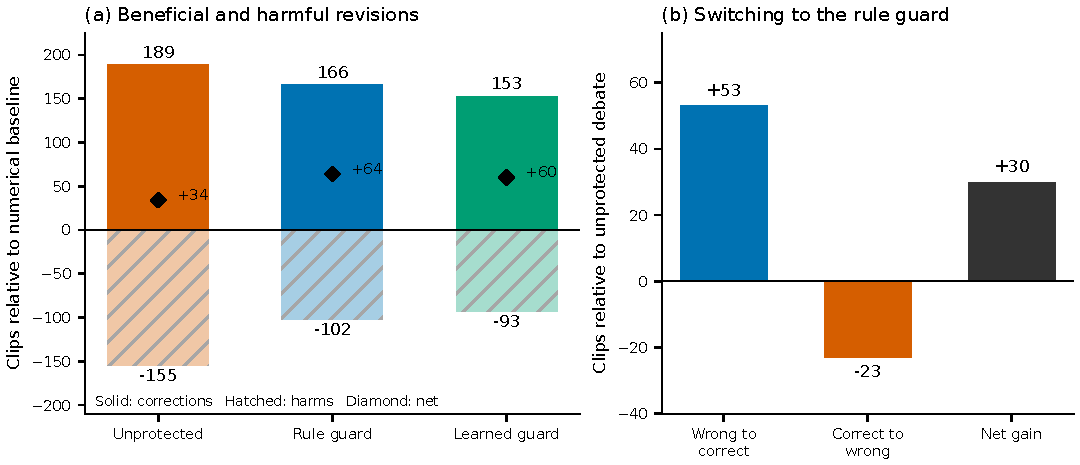
\includegraphics[width=\textwidth]{fig2_correction_benefits_harms.pdf}
\caption{Benefits and harms of baseline-anchored correction on 1,046 clips. (a) Beneficial corrections, harmful revisions, and net corrections relative to the numerical baseline. (b) Paired transitions when replacing unprotected debate with the rule guard: 53 incorrect predictions become correct, while 23 correct predictions become incorrect. Failed protocols retain their prescribed numerical fallback. The reference method differs between panels.}
\label{fig:fig2_correction_benefits_harms}
\end{figure}
\clearpage
\begin{figure}[htbp]
\centering
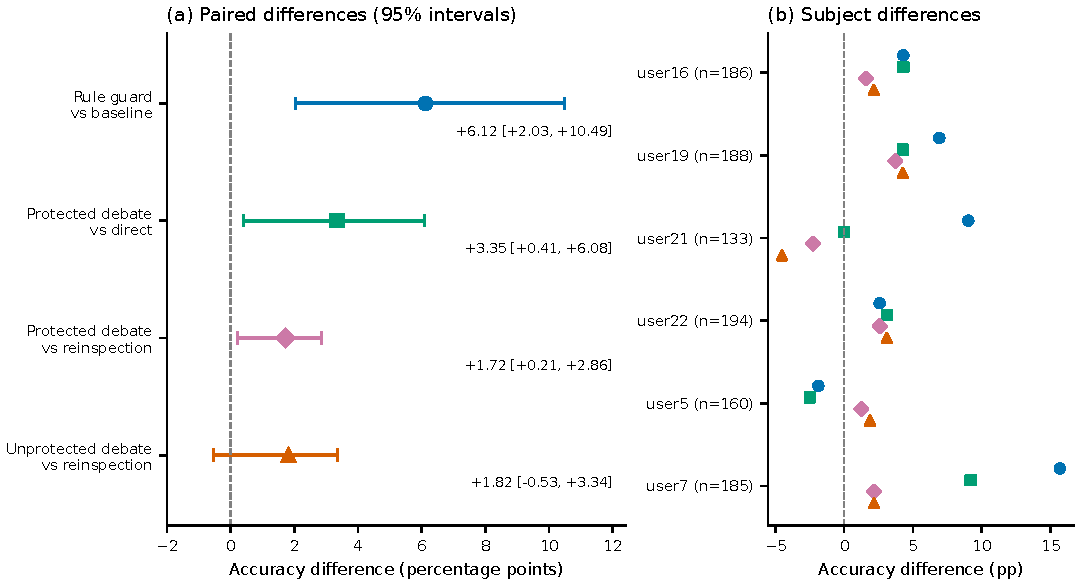
\includegraphics[width=\textwidth]{fig3_paired_differences.pdf}
\caption{Paired accuracy differences and subject-level variability. (a) Point estimates and 95\% subject-clustered bootstrap intervals (2,000 resamples; seed 42). Each difference is the first named method minus the second; direct and reinspection comparators in protected comparisons also use the rule guard. (b) The corresponding differences for each of six subjects, with sample counts. Colors and symbols identify the same comparisons in both panels. Only debate and reinspection are matched at six logical calls; direct arbitration uses three. Intervals are descriptive for this exploratory cohort and do not remove selection bias.}
\label{fig:fig3_paired_differences}
\end{figure}
\clearpage
\begin{figure}[htbp]
\centering
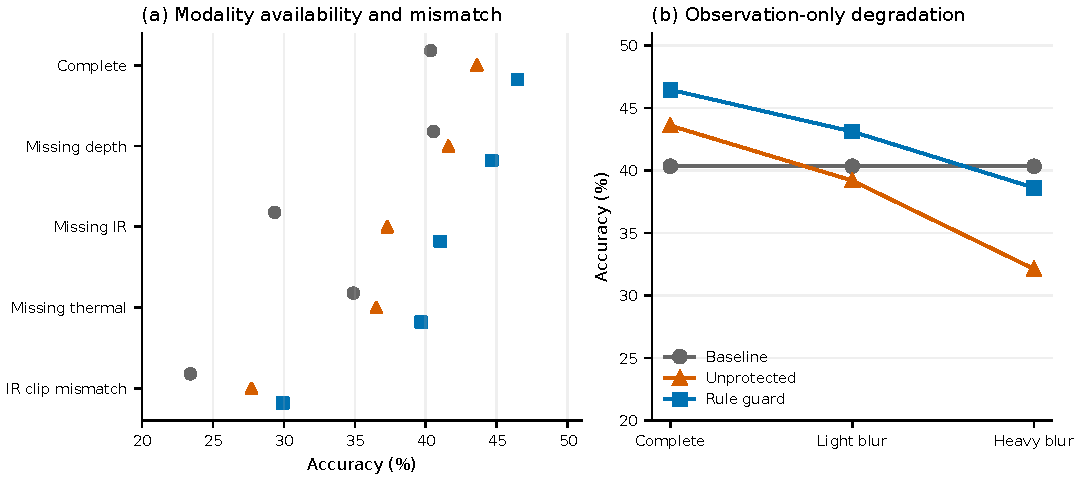
\includegraphics[width=\textwidth]{fig4_input_robustness.pdf}
\caption{Performance under missing, degraded, and mismatched inputs. Each condition contains 1,046 clips. (a) Accuracy under modality removal and synthetic cross-clip IR replacement. (b) Accuracy as agent observations are increasingly blurred. Blur affects only the observation branch, leaving numerical probabilities unchanged. Synthetic IR mismatch is not physical temporal misalignment. Protection mitigates severe-blur damage but remains below the numerical baseline.}
\label{fig:fig4_input_robustness}
\end{figure}
\clearpage
\begin{figure}[htbp]
\centering
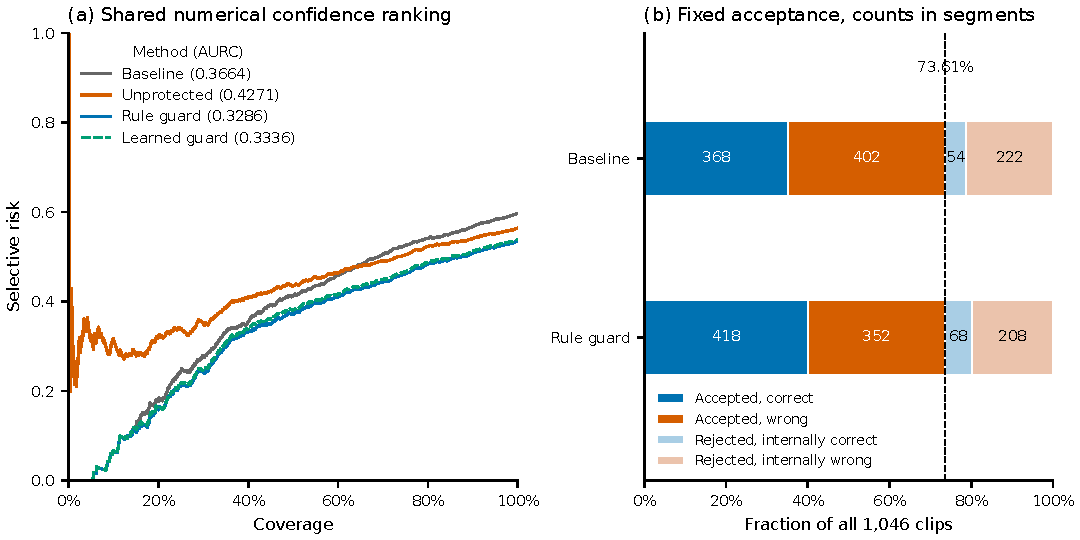
\includegraphics[width=\textwidth]{fig5_selective_prediction.pdf}
\caption{Classification quality and selective prediction. (a) Risk--coverage curves and AURC computed from a shared numerical-confidence ranking, with ties resolved by sample key. Curves do not measure calibration of agent probabilities. (b) Outcome decomposition over all 1,046 clips; numbers within bars are clip counts. Both methods accept the same 770 clips (73.61\% coverage). Correct accepted outputs increase by a net 50, without changing the acceptance set. Rejected outcomes refer to internal predictions.}
\label{fig:fig5_selective_prediction}
\end{figure}
\clearpage
\setcounter{figure}{0}
\renewcommand{\thefigure}{S\arabic{figure}}
\begin{figure}[htbp]
\centering
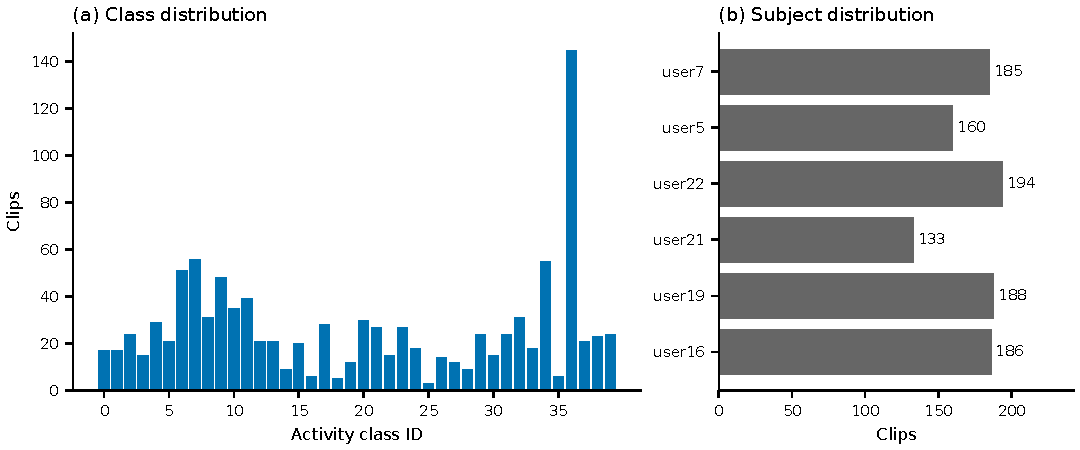
\includegraphics[width=\textwidth]{figS1_cohort_distribution.pdf}
\caption{Distribution of clips across 40 activity classes and six subjects in the 1,046-clip cohort. Activity class IDs follow the prediction-label vocabulary. The class imbalance motivates reporting macro-F1 alongside accuracy.}
\label{fig:figS1_cohort_distribution}
\end{figure}
\clearpage
\begin{figure}[htbp]
\centering
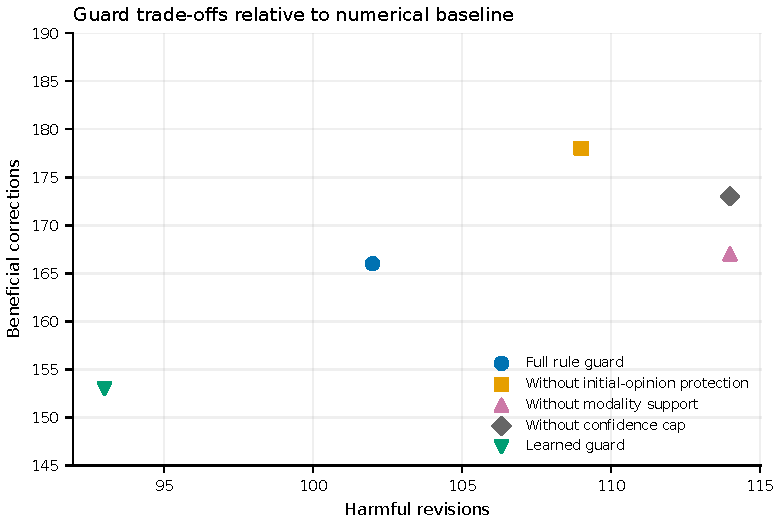
\includegraphics[width=\textwidth]{figS2_guard_tradeoffs.pdf}
\caption{Beneficial corrections versus harmful revisions, each relative to the numerical baseline. Points compare the full rule guard, three single-condition removals, and the learned guard. Higher correction counts and lower harm counts are desirable, but individual constraints trade off both quantities.}
\label{fig:figS2_guard_tradeoffs}
\end{figure}
\clearpage
\begin{figure}[htbp]
\centering
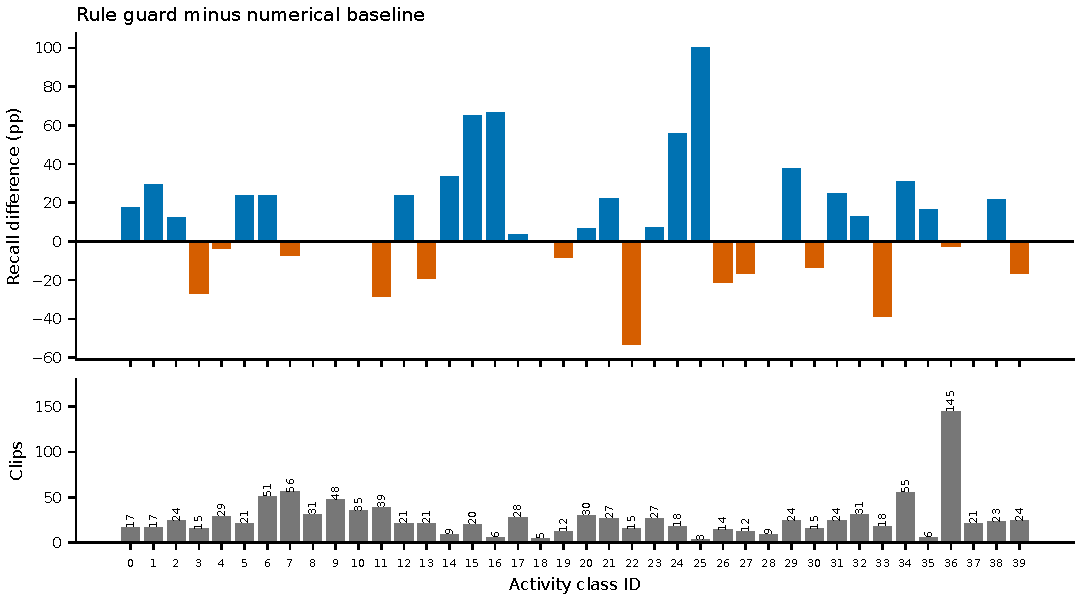
\includegraphics[width=\textwidth]{figS3_class_recall.pdf}
\caption{Class-specific recall changes for the rule guard relative to the numerical baseline, with sample counts below. Differences are in percentage points. Large changes in classes with very few clips, particularly class 25 with three clips, should not be interpreted as stable class-level effects.}
\label{fig:figS3_class_recall}
\end{figure}
\clearpage
\setcounter{table}{3}
\begin{table}[htbp]
\caption{Overall performance on all 1,046 clips. Corrections and harms are relative to the numerical baseline. Missing unimodal predictions count as incorrect; available denominators are 980 (depth), 981 (IR), and 1,019 (thermal). Bold highlights the proposed guarded methods, not column-wise maxima. The rule guard gains 6.12 percentage points over the baseline and reduces harms by 34.2 percent relative to unprotected debate.}
\label{tab:results_main}
\centering\small
\begin{tabular}{@{}lrrrrrr@{}}
\toprule
Method & Correct & Acc. (\%) & Macro-F1 (\%) & Corrections & Harms & Net \\
\midrule
Depth & 255 & 24.38 & 17.83 & 51 & 218 & -167 \\
IR & 370 & 35.37 & 29.97 & 49 & 101 & -52 \\
Thermal & 279 & 26.67 & 18.68 & 51 & 194 & -143 \\
Mean fusion & 404 & 38.62 & 29.53 & 13 & 31 & -18 \\
Baseline & 422 & 40.34 & 31.71 & 0 & 0 & +0 \\
Unprotected & 456 & 43.59 & 36.11 & 189 & 155 & +34 \\
\textbf{Rule guard} & \textbf{486} & \textbf{46.46} & \textbf{37.44} & \textbf{166} & \textbf{102} & \textbf{+64} \\
\textbf{Learned guard} & \textbf{482} & \textbf{46.08} & \textbf{35.82} & \textbf{153} & \textbf{93} & \textbf{+60} \\
\bottomrule
\end{tabular}
\end{table}

\clearpage
\begin{table}[htbp]
\caption{Guard ablations on identical discussion outputs. Corrections and harms are relative to the numerical baseline. Bold identifies the complete proposed rule guard as the reference configuration; ablated variants can achieve higher accuracy.}
\label{tab:results_ablation}
\centering\small
\begin{tabular}{@{}lrrrrrr@{}}
\toprule
Configuration & Correct & Acc. (\%) & Macro-F1 (\%) & Corrections & Harms & Net \\
\midrule
\textbf{Full rule guard} & \textbf{486} & \textbf{46.46} & \textbf{37.44} & \textbf{166} & \textbf{102} & \textbf{+64} \\
Without initial-opinion protection & 491 & 46.94 & 37.60 & 178 & 109 & +69 \\
Without modality support & 475 & 45.41 & 36.70 & 167 & 114 & +53 \\
Without confidence cap & 481 & 45.98 & 37.15 & 173 & 114 & +59 \\
Learned guard & 482 & 46.08 & 35.82 & 153 & 93 & +60 \\
\bottomrule
\end{tabular}
\end{table}

\clearpage
\begin{table}[htbp]
\caption{Controlled observer-model composition on 1,046 clips. All variants use the same distinct observer-role prompts and text auditor. These prompts differ from the primary experiment. Protocol failures are report counts shared by both guard settings, not additional failures caused by protection. Bold highlights accuracy, macro-F1, and harms with the proposed protection in each assignment; it does not indicate the best model assignment.}
\label{tab:model_composition}
\centering\small
\begin{tabular}{@{}lrrrrr@{}}
\toprule
Observer configuration & Acc. (\%) & Macro-F1 (\%) & Corrections & Harms & Failures \\
\midrule
Heterogeneous: Unprotected & 41.68 & 34.59 & 174 & 160 & 14 \\
\textbf{Heterogeneous: Rule guard} & \textbf{45.22} & \textbf{36.43} & 154 & \textbf{103} & 14 \\
Qwen pair: Unprotected & 41.49 & 35.14 & 193 & 181 & 7 \\
\textbf{Qwen pair: Rule guard} & \textbf{45.51} & \textbf{36.67} & 180 & \textbf{126} & 7 \\
Gemma pair: Unprotected & 31.64 & 25.83 & 111 & 202 & 21 \\
\textbf{Gemma pair: Rule guard} & \textbf{35.95} & \textbf{29.58} & 104 & \textbf{150} & 21 \\
\bottomrule
\end{tabular}
\end{table}

\clearpage
\begin{table}[htbp]
\caption{Accuracy under seven input conditions, each with 1,046 clips. Differences compare the rule guard with the same-condition numerical baseline. Intervals use subject-clustered resampling; all differences and interval bounds are in percentage points. Bold highlights the proposed rule guard and its change from the numerical baseline, including the negative change under heavy blur.}
\label{tab:results_robustness}
\centering\small
\begin{tabular}{@{}lrrrrr@{}}
\toprule
Condition & Baseline (\%) & Unprotected (\%) & Rule guard (\%) & Difference & 95\% interval \\
\midrule
Complete & 40.34 & 43.59 & \textbf{46.46} & \textbf{+6.12} & [+2.03, +10.49] \\
Missing depth & 40.54 & 41.59 & \textbf{44.65} & \textbf{+4.11} & [-0.002, +8.62] \\
Missing IR & 29.35 & 37.28 & \textbf{41.01} & \textbf{+11.66} & [+7.19, +14.98] \\
Missing thermal & 34.89 & 36.52 & \textbf{39.67} & \textbf{+4.78} & [+1.48, +8.75] \\
IR clip mismatch & 23.42 & 27.72 & \textbf{29.92} & \textbf{+6.50} & [+1.47, +11.61] \\
Light observation blur & 40.34 & 39.20 & \textbf{43.12} & \textbf{+2.77} & [-1.08, +7.11] \\
Heavy observation blur & 40.34 & 32.12 & \textbf{38.62} & \textbf{-1.72} & [-5.32, +1.95] \\
\bottomrule
\end{tabular}
\end{table}

\clearpage
\end{document}
